% This LMU slides template is adapted from the beaver colortheme by Shengqiang Zhang.
\documentclass{beamer}

\usepackage[utf8]{inputenc}
\usepackage{natbib}
\usepackage{multirow}
\usepackage{booktabs}
\usepackage{float}
\usepackage{bbding}
\usepackage{array}
\usepackage{tikz}
\usetikzlibrary{
  automata, positioning,
  arrows, matrix, decorations.pathreplacing,
  shapes.geometric
}
\usepackage{amsmath,calc}
\let\Tiny\tiny
\beamertemplatenavigationsymbolsempty

\usetheme{Madrid}
% \usetheme{Darmstadt}
% \usetheme{Rochester}
% \usetheme{Frankfurt}
% \usetheme{CambridgeUS}
% \usetheme{default}
% \usefonttheme{serif} %times new roman
\definecolor{Green}{RGB}{43,134,75}
\definecolor{m11}{rgb}{0,48,73}
\definecolor{m12}{rgb}{214,40,40}
\definecolor{m21}{rgb}{247,127,0}
\definecolor{m22}{rgb}{252,191,73}
\usecolortheme{lmugreen}
\setbeamercolor{item projected}{bg=Green,fg=white}
% \definecolor{UBCblue}{rgb}{0.04706, 0.13725, 0.26667} % UBC Blue (primary)

% \usecolortheme[named=LMUGreen]{structure}

\begin{document}
\title[Algebra \& Computer Science]{Formal languages and automatas}
\author[Ruben Triwari]{Ruben Triwari}
\institute[LMU Munich]{
    % \large
    {
\includegraphics[scale=0.032]{images/LMU_Muenchen_Logo.svg.png}} \\
    Seminar: Algebra \& Computer Science, LMU Munich 
}
\date{July 6, 2024}

\tikzset{ 
  table/.style={
    matrix of math nodes,
    row sep=-\pgflinewidth,
    column sep=-\pgflinewidth,
    nodes={rectangle,text width=3em,align=center},
    text depth=1.25ex,
    text height=2.5ex,
    nodes in empty cells,
    left delimiter=[,
    right delimiter={]},
    ampersand replacement=\&
  }
}

% \titlegraphic{
%     \begin{tikzpicture}[remember picture,overlay]
%     \node[anchor=south east, yshift=8pt, xshift=0pt] at (current page.south east)
%     {
\includegraphics[scale=0.032]{images/LMU_Muenchen_Logo.svg.png}};
%     \end{tikzpicture}
% }

\addtobeamertemplate{frametitle}{}{%
\begin{tikzpicture}[remember picture,overlay]
\node[anchor=north east,yshift=8pt, xshift=7pt] at (current page.north east) {
\includegraphics[scale=0.022]{images/LMU_Muenchen_Logo.svg.png}};
\end{tikzpicture}
\vspace{-10pt}
}

\AtBeginSection[]
{
  \begin{frame}
    \frametitle{Outline}
    \tableofcontents[currentsection]
  \end{frame}
}
\frame{\titlepage}
\section{Formal Languages Definitions, Examples}
\begin{frame}
  \frametitle{Alphabets \& Languages}
  An Alphabet $\Sigma$ is a set of characters.\\
  Examples:
  \begin{enumerate}
    \item $\Sigma = \{a,b,c\}$
    \item $\Sigma = \{x\}$
    \item $\Sigma = \emptyset$
  \end{enumerate}
  A Language $L$ is a set of words with characters 
  out of an Alphabet $\Sigma$.\\
  Examples:
  \begin{enumerate}
    \item $\Sigma = \{a,b,c\} \rightsquigarrow L = \{aaa, bbb, ccc, abc\}$
    \item $\Sigma = \{x\} \rightsquigarrow L = \{ x, xx, xxx, xxxx\}$
    \item $\Sigma = \emptyset \rightsquigarrow L = \{\epsilon \}$
  \end{enumerate}
  $\rightsquigarrow L \subset \Sigma^*$
\end{frame}

\begin{frame}
  \frametitle{Formal series}
  We can also write a Language with a formal series, with a fixed $\Sigma$:
    \[ L = \sum (L,w)w\]
    \[ 
      \leftrightsquigarrow  L = 
      \bigcup_{w \in \Sigma^{*}}
      \underbrace{(L,w)}_\text{0 or 1}
      \{w\} 
    \]
  Examples:
  \begin{enumerate}
    \item $\Sigma = \{a,b,c\} \rightsquigarrow L = \{aaa, abc\}$ \\
          $\rightsquigarrow L = 1aaa + 1abc + 0a + 0b + 0c + \dots$
    \item $\Sigma = \{x\} \rightsquigarrow L = \{ x, xx\}$ \\
            $\rightsquigarrow L = 1x + 1xx + 0xxx + 0xxxx +  0xxxxx + \dots$
          \item $\Sigma = \emptyset \rightsquigarrow L = \{ \epsilon \}$ \\
            $\rightsquigarrow L = 1\epsilon$
  \end{enumerate}
\end{frame}

\begin{frame}
  \frametitle{Addition}
    Now we can define Addition on formal series:
  \[ U + V = \sum (\underbrace{(U,w) + (V,w)}_\text{Boolean addition})w\]
  \[\leftrightsquigarrow  U + V = U \cup V\] 
  Exmaple:\\
  Let $U = \{x, xx\}$ and $V = \{aaa, abc\}$ languages:
  \begin{align*} 
    U + V &= (1+0)x + (1+0)xx + (0+1)aaa + (0+1)abc  + (0+0)a + \dots \\
          &= 1x + 1xx + 1aaa + 1abc + 0a + \dots
  \end{align*}
\end{frame}

\begin{frame}
  \frametitle{Multiplication}
  Next we can define multiplication on formal series:
    \[
      U \cdot V = \sum (\underbrace{(U,s) \cdot (V,t)}_\text{Boolean multiplication})w
      \text{, such that  } st = w
    \]
    \[\leftrightsquigarrow U \cdot V = \{\ st \text{ } | \text{ } s \in U \land t \in V \} \]

  Exmaple:\\
  Let $U = \{x, xx\}$ and $V = \{aaa, abc\}$ languages:
  \begin{align*} 
    U \cdot V &= (1\cdot1)xaaa + (1\cdot1)xxaaa + (1\cdot1)xabc 
    + (1\cdot1)xxabc  \\ &\hspace{2cm} + (0\cdot0)axxx + \dots \\
              &= 1xaaa + 1xxaaa + 1xabc + 1xxabc  + 0axxx + \dots 
  \end{align*}
\end{frame}

\begin{frame}
  \frametitle{Algebra \& Kleene Star}
  With these definitions, all languages with a fixed alphabet $\Sigma$
  form an algebra $\mathbb{B}\langle \Sigma \rangle $ over $\mathbb{B}$.\\
  \vspace*{1cm}
  {\bf Kleene star:} \\
  Let $U$ be a Language.\\
  \[ U^* = \epsilon + U + U^2 + U^3 + \dots \]

  Exmaple:\\
  Let $U = x$.
  \[ U^* = \epsilon + x  + x^2 + x^3 + x^4 + \dots \]

  
\end{frame}

\section{Prove not all Languages are rational (regular)}
\begin{frame}
  \frametitle{Rational Languages}
  All languages generated by a finite number of additions, multiplications, 
  and kleene star is a rational (regular) language.\\
  {\bf Examples:}\\
  $\Sigma = \{x, y, z\}$ 
  \begin{align}
    L_1 &= x+y \\
    L_2 &=(x+y+z)^* \\
    L_3 &= (x+y^*)^*z^*\\
    L_4 &=(xyz)^*(y+x^*zxyx^*)^*
  \end{align}
\end{frame}
\begin{frame}
  \frametitle{Gaps in rational languages}
  {\bf We show that not all languages generated 
  by a single letter are rational}.\\
  Let $L_x = x$.\\
  A gap in a language generated by $L_x$ is the
  amount of consecutive missing powers.\\
  {\bf Examples:}\\
  \begin{align*}
    L_1 &= x \rightsquigarrow gaps(L_1) = \{0\} \\ 
    L_2 &= x + x^2 + x^3 \rightsquigarrow gaps(L_2) = \{0\} \\
    L_3 &= x + x^5 + x^7 \rightsquigarrow gaps(L_3) = \{0,3,1\} \\
    L_4 &= x + x^5 + x^7 \rightsquigarrow maxgap(L_4) = 3
  \end{align*}
\end{frame}
\begin{frame}
  \frametitle{Intuition of the proof}
  {\bf Raional languages generated by x have alway a finite maximum gap.}
  
  {\bf Examples of not rational languages:}\\
  \begin{align*}
    L_1 &= x + x^2 + x^4 + x^7 + x^{11} 
    \dots \rightsquigarrow gaps(L_1) = \{0,1,2,3, \dots\} \\ 
    L_2 &= x^3 + x^{31} + x^{314} + x^{3141} \dots
    \rightsquigarrow gaps(L_2) = \{27, 282, 2826, \dots\} \\
  \end{align*}
  $\rightsquigarrow$ Only way to get an endless sequence is
    using the star operator.\\
  $\rightsquigarrow$ The star operator just repeats the language
  an abritary amount of times\\
  $\rightsquigarrow$ Informally we can say rational languages are finite or have an repeating pattern.
\end{frame}

\begin{frame}
  \frametitle{Proof sketch}
  Claim: {\bf
    All rational languages generated by $L_x$ have a
    maximum gap
  }\\
  Let L be language generated by $L_x$
  \[ maxgap(L) < \infty. \]
  {\bf Structural induction over $+, \cdot, ^*$:}\\
  \vspace{1cm}
  Base case: \\
  \[L = L_x = x\]
  \[ \implies maxgap(L) = maxgap(L_x) = maxgap(x) = 0\]
\end{frame}
\begin{frame}
  \frametitle{Proof sketch}
  {\bf Addition case:}\\
  Let $L_1,L_2$ languages generated by $L_x$ with a maximum gap.\\
  We need to show that: 
  \[ maxgap(L_1+L_2) < \infty \]\\
  \[ L_1 = x^a + x^b + x^c + x^d + \dots  \]
  \[ L_2 = x^k + x^l + x^m + x^n + \dots  \]
  \vspace{0.05cm}
  \[ \downarrow \]
  \vspace{0.05cm}
  \begin{center}
    \begin{tikzpicture}
      \draw[->] (-4.5,0) -- (5.5,0) ; %edit here for the axis
      \foreach \x in  {-4,-3,-2,-1,0,1,2,3,4, 5} % edit here for the vertical lines
      \draw[shift={(\x,0)},color=black] (0pt,3pt) -- (0pt,-3pt);
      \node[] at (-3,-0.5) {a};
      \node[] at (-2,-0.5) {k};
      \node[] at (-1,-0.5) {l};
      \node[] at (0,-0.5) {b};
      \node[] at (1,-0.5) {m};
      \node[] at (2,-0.5) {c};
      \node[] at (3,-0.5) {d};
      \node[] at (4,-0.5) {n};
      \node[] at (5,-0.5) {$\dots$};
    \end{tikzpicture}
  \end{center}
\end{frame}
\begin{frame}
  \frametitle{Proof sketch}
  {\bf case 1:  The series of their powers intersect}\\
  \vspace{0.05cm}
  \begin{center}
    \begin{tikzpicture}
      \draw[->] (-4.5,0) -- (5.5,0) ; %edit here for the axis
      \foreach \x in  {-4,-3,-2,-1,0,1,2,3,4, 5} % edit here for the vertical lines
      \draw[shift={(\x,0)},color=black] (0pt,3pt) -- (0pt,-3pt);
      \node[] at (-3,-0.5) {a};
      \node[] at (-2,-0.5) {k};
      \node[] at (-1,-0.5) {l};
      \node[] at (0,-0.5) {b};
      \node[] at (1,-0.5) {m};
      \node[] at (2,-0.5) {c};
      \node[] at (3,-0.5) {d};
      \node[] at (4,-0.5) {n};
      \node[] at (5,-0.5) {$\dots$};
    \end{tikzpicture}
  \end{center}
  $\rightsquigarrow $ Gaps are only getting filled
  $\rightsquigarrow maxgap(L_1+L_2) \le max(maxgap(L_1), maxgap(L_2))$ \\
  \vspace{1cm}
  {\bf case 2:  The series of their powers don't intersect}\\
  \vspace{0.05cm}
  \begin{center}
    \begin{tikzpicture}
      \draw[->] (-5.5,0) -- (6.5,0) ; %edit here for the axis
      \foreach \x in  {-5,-4,-3,-2,-1,0,1,2,3,4,5,6} % edit here for the vertical lines
      \draw[shift={(\x,0)},color=black] (0pt,3pt) -- (0pt,-3pt);
      \node[] at (-5,-0.5) {a};
      \node[] at (-4,-0.5) {b};
      \node[] at (-3,-0.5) {c};
      \node[] at (-2,-0.5) {$\dots$};
      \node[] at (-1,-0.5) {z};
      \node[] at (1,-0.5) {k};
      \node[] at (2,-0.5) {l};
      \node[] at (3,-0.5) {m};
      \node[] at (4,-0.5) {n};
      \node[] at (5,-0.5) {$\dots$};
    \end{tikzpicture}
  \end{center}
  \[\rightsquigarrow maxgap(L_1+L_2) \le max(
        max(maxgap(L_1), maxgap(L_2)),
      k-z+1)\] \\
\end{frame}

\begin{frame}
  \frametitle{Proof sketch}
  {\bf Multiplication case:}\\
  Let $L_1,L_2$ languages generated by $L_x$ with a maximum gap.\\
  We need to show that: 
  \[ maxgap(L_1 \cdot L_2) < \infty \]\\
  \[ L_1 = x^a + x^b + x^c + x^d + \dots  \]
  \[ L_2 = x^k + x^l + x^m + x^n + \dots  \]
  \vspace{0.05cm}
  \[ L_1 \cdot L_2 = x^{a+k} + x^{a+l} +  \dots +x^{b+k} + x^{b+l}+ \dots \]\\
  \[ \downarrow \]
  \vspace{0.05cm}
  \begin{center}
    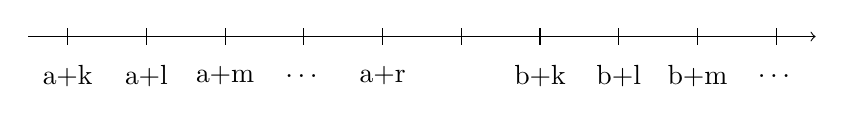
\begin{tikzpicture}
      \draw[->] (-5.5,0) -- (4.5,0) ; %edit here for the axis
      \foreach \x in  {-5,-4,-3,-2,-1,0,1,2,3,4} % edit here for the vertical lines
      \draw[shift={(\x,0)},color=black] (0pt,3pt) -- (0pt,-3pt);
      \node[] at (-5,-0.5) {a+k};
      \node[] at (-4,-0.5) {a+l};
      \node[] at (-3,-0.5) {a+m};
      \node[] at (-2,-0.5) {$\dots$};
      \node[] at (-1,-0.5) {a+r};
      \node[] at (1,-0.5) {b+k};
      \node[] at (2,-0.5) {b+l};
      \node[] at (3,-0.5) {b+m};
      \node[] at (4,-0.5) {$\dots$};
    \end{tikzpicture}
  \end{center}
\end{frame}
\begin{frame}
  \frametitle{Proof sketch}
  {\bf case 1:  The groups don't intersect}\\
  \vspace{0.05cm}
  \begin{center}
    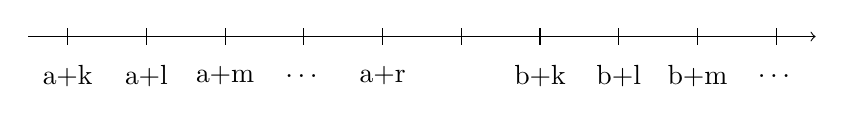
\begin{tikzpicture}
      \draw[->] (-5.5,0) -- (4.5,0) ; %edit here for the axis
      \foreach \x in  {-5,-4,-3,-2,-1,0,1,2,3,4} % edit here for the vertical lines
      \draw[shift={(\x,0)},color=black] (0pt,3pt) -- (0pt,-3pt);
      \node[] at (-5,-0.5) {a+k};
      \node[] at (-4,-0.5) {a+l};
      \node[] at (-3,-0.5) {a+m};
      \node[] at (-2,-0.5) {$\dots$};
      \node[] at (-1,-0.5) {a+r};
      \node[] at (1,-0.5) {b+k};
      \node[] at (2,-0.5) {b+l};
      \node[] at (3,-0.5) {b+m};
      \node[] at (4,-0.5) {$\dots$};
    \end{tikzpicture}
  \end{center}
  $\rightsquigarrow $ Gaps in one group stay the same\\
  $\rightsquigarrow$ For gaps between groups hold: 
    \[b+k - (a+r) = b-a + k-r \le maxgap(L_1) + 0 = maxgap(L_1)\]
  \[\rightsquigarrow maxgap(L_1\cdot L_2) \le  max(maxgap(L_1),maxgap(L_2))\] \\
  \vspace{1cm}
  {\bf case 2:  The groups intersect}\\
  \vspace{0.05cm}
  \begin{center}
    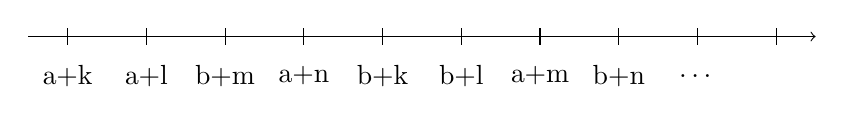
\begin{tikzpicture}
      \draw[->] (-5.5,0) -- (4.5,0) ; %edit here for the axis
      \foreach \x in  {-5,-4,-3,-2,-1,0,1,2,3,4} % edit here for the vertical lines
      \draw[shift={(\x,0)},color=black] (0pt,3pt) -- (0pt,-3pt);
      \node[] at (-5,-0.5) {a+k};
      \node[] at (-4,-0.5) {a+l};
      \node[] at (-3,-0.5) {b+m};
      \node[] at (-2,-0.5) {a+n};
      \node[] at (-1,-0.5) {b+k};
      \node[] at (0,-0.5) {b+l};
      \node[] at (1,-0.5) {a+m};
      \node[] at (2,-0.5) {b+n};
      \node[] at (3,-0.5) {$\dots$};
    \end{tikzpicture}
  \end{center}
  \[\rightsquigarrow maxgap(L_1\cdot L_2) \le max(maxgap(L_1), maxgap(L_2))\] \\
\end{frame}
\begin{frame}
  \frametitle{Proof sketch}
  {\bf Kleene star case:}\\
  Let $L$ be a language generated by $L_x$ with a maximum gap.\\
  We need to show that: 
  \[ maxgap(L^*) < \infty \]\\
  \vspace{1cm}
  It's easy to see with induction: 
  \[\forall n \in \mathbb{N}_0: maxgap(L^n) \le maxgap(L)\]
  \vspace{0.5cm}
  \[\rightsquigarrow L^* = \underbrace{
      \underbrace{\epsilon}_{\le maxgap(L)} +
      \underbrace{L}_{\le maxgap(L)} +
      \underbrace{L^2}_{\le maxgap(L)} +
      \underbrace{L^3}_{\le maxgap(L)}+ 
      \underbrace{L^4}_{\le maxgap(L)} + \dots
    }_{\le maxgap(L)}\]
  \vspace{0.05cm}
\end{frame}
\section{Automatas Definitions, Examples}
\begin{frame}[fragile]
  \frametitle{Automatas and transistion matrices}
  \begin{center}
    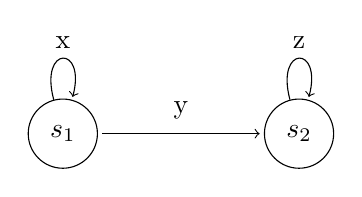
\begin{tikzpicture}
      \node[state] (q1) at (0,0) {$s_1$};
      \node[state] (q2) at (3,0) {$s_2$};
      \draw (q1) edge[loop above] node{x} (q1)
      (q2) edge[loop above] node{z} (q2);
      \draw[->](0.5,0)--(2.5,0);
      \node[fill=white] at (1.5,0.3) {y};
    \end{tikzpicture}
    \\
    \vspace{0.5cm}
    $\downarrow$\\
    \vspace{0.5cm}
    \begin{tikzpicture}[baseline,decoration=brace]
        \matrix (m) [table] {
          x \& y \\
          0 \& z \\
        };
      \node[fill=white] at (-2,0.4) {$s_1$};
      \node[fill=white] at (-2,-0.4){$s_2$};

      \node[fill=white] at (-0.7,-1.5){$s_1$};
      \node[fill=white] at (0.7,-1.5) {$s_2$};
    \end{tikzpicture}
  \end{center}
\end{frame}
\begin{frame}
  \frametitle{Automatas and transistion matrices}
  {\bf Formally, we can write:}\\
  Let $S = \{s_1, s_2, \dots, s_n\}$, $A \in (\Sigma^*)^{n \times n}$.\\
  Then a transition from state $s_1$ to $s_2$:\\
  \[ s_iA_{ij} = s_j\]
  
  Exmaple:\\
  Let $S = \{s_1, s_2\}$ and $ A = 
  \begin{pmatrix}
    x & y \\
    0 & z 
  \end{pmatrix}
  $
  \begin{align*}
    s_1A_{11} &= s_1x = s_1 \\
    s_1A_{12} &= s_1y = s_2 \\
    s_2A_{22} &= s_2z = s_2 \\
  \end{align*}
\end{frame}


\begin{frame}
  \frametitle{Matrix multiplication and transistion matrices}
  {\bf What happends if we apply matrix multiplication on 
  $A \in (\Sigma^*)^{n \times n}$?}
  \begin{equation*}
    \begin{aligned}
      C = A^1: \hspace{0.5cm} c_{ij} &= a_{ij}
      \rightsquigarrow 
      \text{from state i to state j in 1 steps}\\
      C = A^2: \hspace{0.5cm} c_{ij} &= \sum_{k=1}^{n} a_{ik}a_{kj}
      \rightsquigarrow 
      \text{from state i to state j in 2 steps}\\
      C = A^3: \hspace{0.5cm} c_{ij} &= \sum_{k_1=1}^{n}
      \sum_{k_2=1}^{n}a_{ik_1}a_{k_1k_2}a_{k_2j} \rightsquigarrow 
      \text{from state i to state j in 3 steps}\\ 
                          &\vdots\\
      C = A^n: \hspace{0.5cm} c_{ij} &= \sum_{k_1=1}^{n}
      \sum_{k_2=1}^{n}\dots \sum_{k_{n-1}=1}^n 
      a_{ik_1}a_{k_1k_2}\dots a_{k_{n-2}k_{n-1}}a_{k_{n-1}j} \\
        &\rightsquigarrow \text{from state i to state j in n steps}\\ 
    \end{aligned}
  \end{equation*}
\end{frame}

\begin{frame}
  \frametitle{Kleene star and transistion matrices}
  {
    \bf Combining these will give us all possible 
    inputs from one state in another:
  }

  \begin{equation*}
    \begin{aligned}
      A^* &= E_n + A + A^2 + A^3+ \dots \\
      A^* &= \sum_{k \in \mathbb{N}_0} A^k\\
    \end{aligned}
  \end{equation*}
  $\rightsquigarrow \text{ In } a_{ij} \in A$ are all possible inputs
   carrying state i to state j in any \\
   \hspace{0.5cm} abitrary amount of steps.
\end{frame}
\section{Prove: Finite automaton only accept rational languages}
\begin{frame}
  \frametitle{Prove sketch}
  Let $M \in (\Sigma^*)^{n\times n}$ an abritary transition matrix with rational
  entries.\\
  We need to show that every entry of $M^*$ is rational.\\
  {\bf Devide the matrix in the following block matrices.}\\
  \[M = 
    \begin{pmatrix}
      M(1,1) & M(1,2) \\
      M(2,1) & M(2,2)
    \end{pmatrix} 
    \in (\Sigma^*)^{n\times n}
  \]
  Where: \\
  \[
    \textcolor{brown}{M(1,1) \in (\Sigma^*)^{1\times 1}},
    \textcolor{blue}{M(1,2) \in (\Sigma^*)^{1\times n-1}}
  \]
  \[
    \textcolor{orange}{M(2,1) \in (\Sigma^*)^{n-1\times 1}},
    \textcolor{red}{M(2,2) \in (\Sigma^*)^{n-1\times n-1}}
  \]
  \begin{center}
    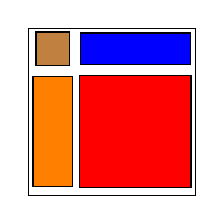
\begin{tikzpicture}[square/.style={regular polygon,regular polygon sides=4}]
        \node at (0,0) [square,draw,minimum width=3cm] (m) {};
        \node at (0.3,0.8) [rectangle,draw,minimum height=0.4cm,minimum width=1.4cm,fill=blue] (m21) {};
        \node at (-0.75,-0.25) [rectangle,draw,minimum height=1.4cm,minimum width=0.5cm,fill=orange] (m12) {};
        \node at (0.3,-0.25) [square,draw,minimum width=2cm,fill=red] (m) {};
        \node at (-0.75,0.8) [square,draw,minimum width=0.6cm,fill=brown] (m) {};
    \end{tikzpicture}
  \end{center}
\end{frame}
\begin{frame}
  We can devide the all States $S = \{s_1,s_2,\dots,s_n\}$
  in two:
  \[1 = \{s_1\} \text{ and } 2 = \{s_2,s_3, \dots ,s_n\}\]
  {\bf Automata with devided transition matrix and states:}
  \begin{center}
    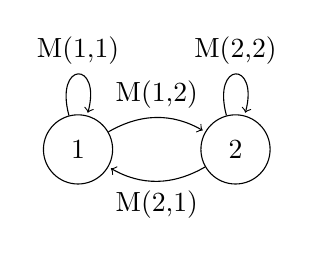
\begin{tikzpicture}[shorten >=1pt,node distance=2cm,on grid,auto] 
       \node[state] (q_0)   {$1$}; 
       \node[state](q_1) [right=of q_0] {$2$};
        \path[->] 
        (q_0) edge[bend left, above]  node {M(1,2)} (q_1)
              edge [loop above] node {M(1,1)} ()
        (q_1) edge[bend left, below]  node {M(2,1)} (q_0)
              edge [loop above] node {M(2,2)} ();
    \end{tikzpicture}
  \end{center}
\end{frame}
\begin{frame}
  \frametitle{Proof sketch}
  {\bf We can write $M^*$ in terms of our block matrices:}
  \[ M(1,1)^* = M(1,1)^*+(M(1,2)M(2,2)^*M(2,1))^*\]
  \[ M(1,2)^* = M(1,1)^*M(1,2)(M(2,2)^* + M(2,1)M(1,1)^*M(1,2))^*\]
  \[ M(2,1)^* = M(2,2)^*M(2,1)(M(1,1)^* + M(1,2)M(2,2)^*M(2,1))^*\]
  \[ M(2,2)^* = M(2,2)^*+(M(2,1)M(1,1)^*M(1,2))^*\]
  \vspace{0.5cm}
  \begin{center}
    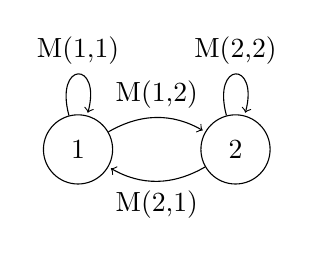
\begin{tikzpicture}[shorten >=1pt,node distance=2cm,on grid,auto] 
       \node[state] (q_0)   {$1$}; 
       \node[state](q_1) [right=of q_0] {$2$};
        \path[->] 
        (q_0) edge[bend left, above]  node {M(1,2)} (q_1)
              edge [loop above] node {M(1,1)} ()
        (q_1) edge[bend left, below]  node {M(2,1)} (q_0)
              edge [loop above] node {M(2,2)} ();
    \end{tikzpicture}
  \end{center}
\end{frame}
\begin{frame}
  \frametitle{Proof sketch}
  {\bf We have reduced the problem to $n-1$:}
  \[ M(1,1)^* = M(1,1)^*+(M(1,2)M(2,2)^*M(2,1))^*\]
  \[ M(1,2)^* = M(1,1)^*M(1,2)(M(2,2)^* + M(2,1)M(1,1)^*M(1,2))^*\]
  \[ M(2,1)^* = M(2,2)^*M(2,1)(M(1,1)^* + M(1,2)M(2,2)^*M(2,1))^*\]
  \[ M(2,2)^* = M(2,2)^*+(M(2,1)M(1,1)^*M(1,2))^*\]\\
  \vspace{0.5cm}
  $\rightsquigarrow M(1,1)^*$ is rational, because its 1-dimensional\\
  $\rightsquigarrow M(2,1), M(1,2)$ is rational, because $M$ is rational\\
  $\rightsquigarrow M(2,2)^* \in (\Sigma^*)^{(n-1) \times (n-1)}$ 
    needs to be proven, to be rational \\
  $\rightsquigarrow $ With this reduction we can do an induction over the number of states
\end{frame}



\begin{frame}
    \Huge{\centerline{Thanks for your attention!}}
    % \Huge{\centerline{Any Questions?}}
    
\end{frame}



\bibliography{references}
\bibliographystyle{acl_natbib}
\end{document}
